\documentclass{article}

% Language setting
% Replace `english' with e.g. `spanish' to change the document language
\usepackage[english]{babel}

\mathchardef\mathcomma=\mathcode`,
% Set page size and margins
% Replace `letterpaper' with `a4paper' for UK/EU standard size
\usepackage[letterpaper,top=2cm,bottom=2cm,left=3cm,right=3cm,marginparwidth=1.75cm]{geometry}

% Useful packages
\usepackage{amsmath}
\usepackage{graphicx}
\usepackage[colorlinks=true, allcolors=blue]{hyperref}
%\theoremstyle{definition}
\usepackage{hyperref} 
\newtheorem{definition}{Definition}[section]
\usepackage{cite}
\usepackage{amsmath,amssymb,amsfonts}
\usepackage{algorithmic}
\usepackage{graphicx}
\usepackage{textcomp}
\usepackage{xcolor}
\usepackage{subcaption}
\usepackage{svg}
\graphicspath{ {./images/} }
\usepackage{float}
\usepackage{placeins}
\usepackage{tablefootnote}


\title{Network Dynamics Homework II}
\author{ Minh Triet Ngo(s309062)}

\begin{document}
\date{17 December, 2023}
\maketitle

\section{Exercise 1}
\subsection{a}
\textit{What is according to the simulations, the average time it takes a particle that
starts in node b to leave the node and the return to it?} \\
The average return time according to the simulation is 4.6
\subsection{b}
\textit{How does the result in a) compare to the theoretical return time} $E_b[T_b^+]$\textit{?(include a description of how it is computed)} \\
The theoretical expected return time can be computed by the following formula given the assumptions stated in \textbf{Theorem 7.2}\\
$$E_i[\bar{T}_i^+] = \frac{1}{\omega_i\bar{\pi}_i}$$ 
The result shows that the simulation agrees with theoretical value.
\subsection{c}
\textit{What is, according to the simulation, the average time it takes to move from node o to node d?}\\
The average time for a particle to move from node o to node d is 10.8.
\subsection{d}
\textit{How does the result ub c) compare to the theoretical hitting-time} $E_o[T_d]$\textit{? (Describe also how this is computed)}\\
The expected hitting time can be computed according to \textbf{Theorem 7.2} by solving following system.
$$\bar{\tau}_i^{\mathcal{S}} = E_i[T_{\mathcal{S}}], \quad i \in \mathcal{X} $$
are the unique solution of
$$\bar{\tau}_s^{\mathcal{S}} = 0, \quad s \in \mathcal{S}, \quad \quad \bar{\tau}_i^{\mathcal{S}} = \frac{1}{\omega_i} + \sum_{j \in \mathcal{X} }P_{ij}\bar{\tau}_j^{\mathcal{S}}, \quad i \in \mathcal{X} \setminus \mathcal{S}$$
The simulation agrees with the theoretical value.
\subsection{e}
The dynamic converge to a consensus because graph $\mathcal{G}$ is strongly connected and aperiodic.
\subsection{f}
Consensus variance can be computed by the dot product between by stationary distribution of normalized weight matrix $\pi$ and the vector of variances
$$\sigma^2 = \sum_{i \in \mathcal{V}}\pi_i\sigma_i^2$$
The result is 0.259 which agrees with the estimation.
\subsection{g}
After removing (d,a), (d,c) node d become the unique sink of $\mathcal{G}$
\begin{figure}[!htbp]
    \centering
    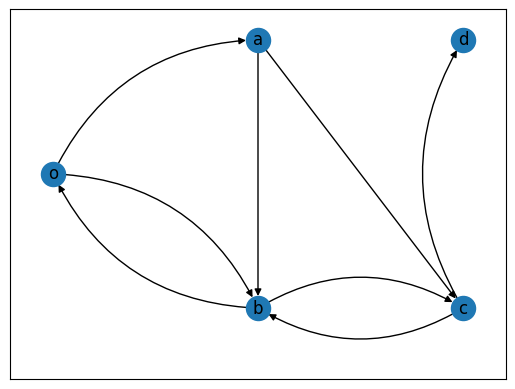
\includegraphics[width=\linewidth]{fig/1g}   
    \caption{new graph}
   \label{fig:figure1}
\end{figure}

\begin{figure}[!htbp]
    \centering
    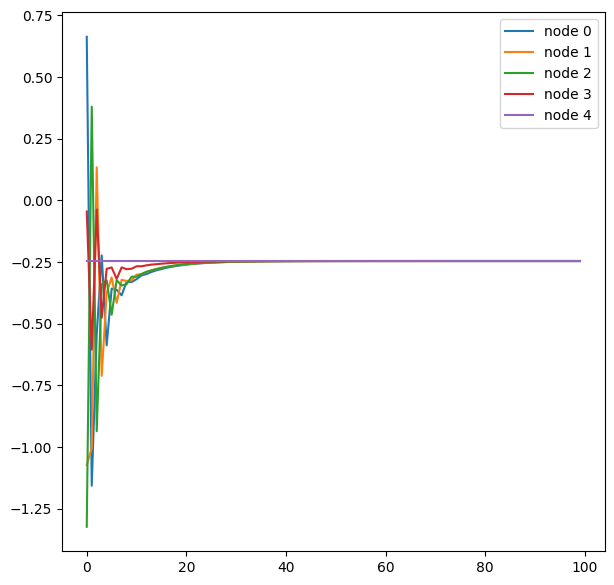
\includegraphics[width=\linewidth]{fig/consensus_converge}   
    \caption{consensus converge}
   \label{fig:figure2}
\end{figure}

This can be consider as a distributed averaging model of stubborn node. In this case the consensus converge to the initial value of node d.
We know that the stationary distribution of the normalized weight matrix is supported on sink node only thefore the variance of consensus value 
is the same with the variance of node d

\subsection{h}
After removing (c,b),(d,a) graph $\mathcal{G}$ is no longer strongly connected and the sink component is periodic 
and for that reason the consensus does not converge. The initial value of nodes in sink component does not change but exchange step by step.

\begin{figure}[!htbp]
    \centering
    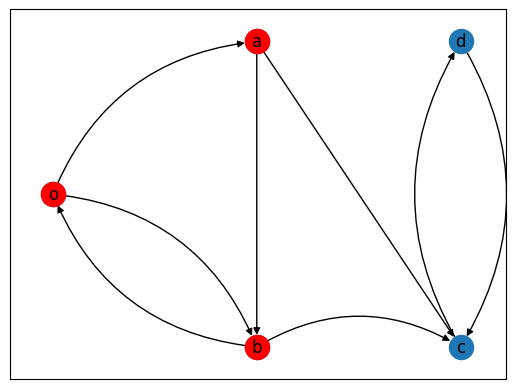
\includegraphics[width=\linewidth]{fig/1h}   
    \caption{new graph}
   \label{fig:figure100}
\end{figure}

\begin{figure}[!htbp]
    \centering
    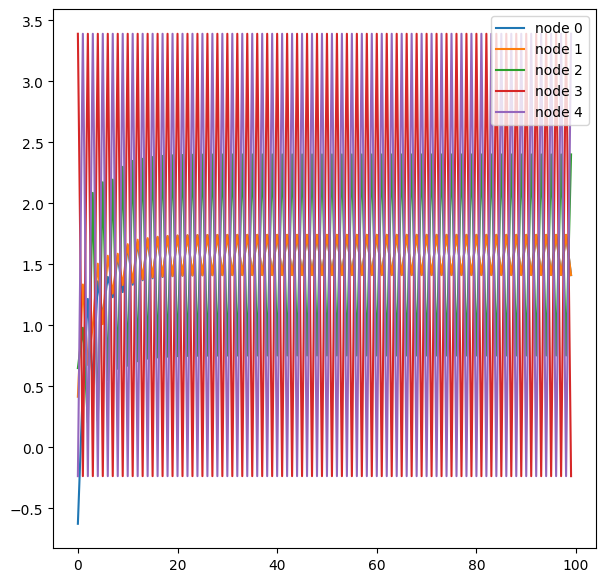
\includegraphics[width=\linewidth]{fig/consensus_notconverge}   
    \caption{consensus not converge}
    \label{fig:figure3}
\end{figure}

\section{Ex2}
\subsection{a - Particla perspective}
The average time for a particle to return to node b is around 4.6 which is the same 
in comparison with the value in Ex1. The value can be explained by the indepence in movement of the particles in the sense that
the movements of 100 particles are equivalent to the movement of a particle repeated 100 times.
\subsection{b - Node perspective}
After the initial transitory phase, the average number of particles at node o,a,b,c,d is respectively 21.78, 14.9, 27.09, 17.95, 18.23.
The result is approximately equivalent to the stationary distribution.

\begin{figure}[!htbp]
    \centering
    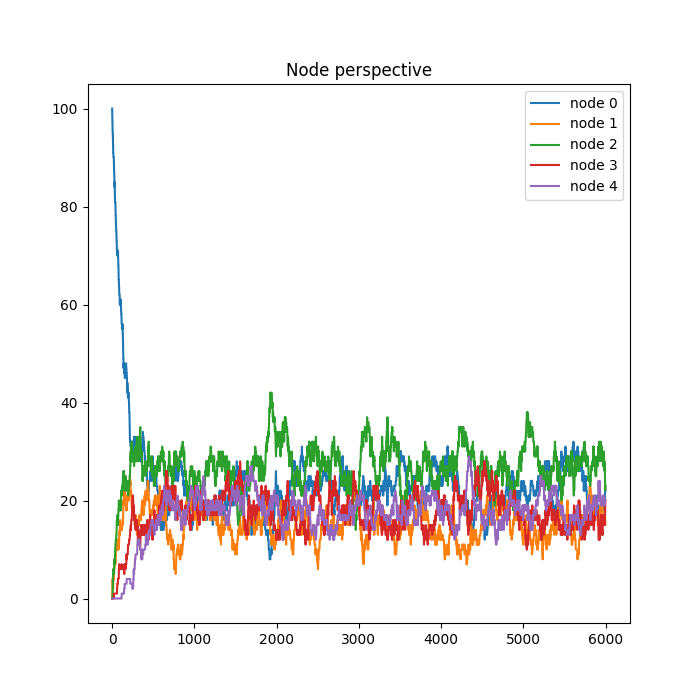
\includegraphics[width=\linewidth]{fig/node_perspective}   
    \caption{number of particles at nodes in simulation}
    \label{fig:figure4}
\end{figure}

\section{Ex3}
\subsection{a - Proportional rate}
Each node in the network can be thought of as a M/M/$\infty$ queue and theoretically we know an M/M/$\infty$ does not blow up. We run another simulation
with input rate of 200 and the number of particles at each node increase but not too much.
\begin{figure}[!htbp]
    \centering
    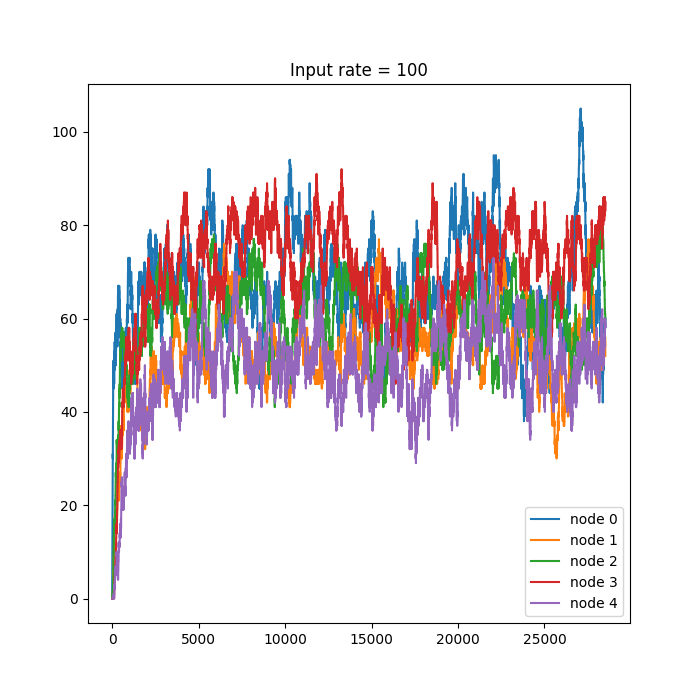
\includegraphics[width=\linewidth]{fig/proportional_100}   
    \caption{number of particles at nodes in simulation}
    \label{fig:figure5}
\end{figure}

\begin{figure}[!htbp]
    \centering
    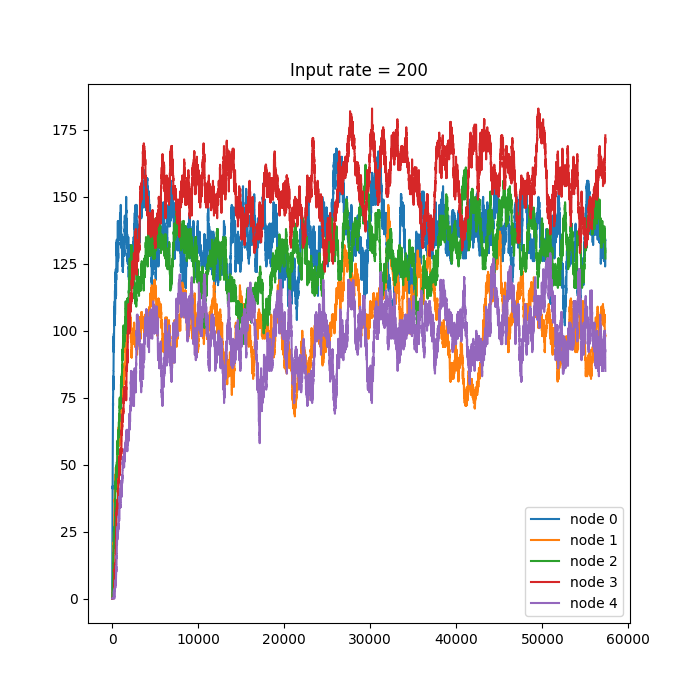
\includegraphics[width=\linewidth]{fig/proportional_200}   
    \caption{number of particles at nodes in simulation}
    \label{fig:figure6}
\end{figure}


\subsection{b - Fixed rate}
Each node of the graph can be thought of as an M/M/1 queue and we know that for such a queue to be stable
the ratio between the input rate and the output rate must be smaller than 1. It is easy to see that node o is the first one to be blowing up
with increasing input rate as shown in three simulations below with input rate = 0.5, 1, 2.

\begin{figure}[!htbp]
    \centering
    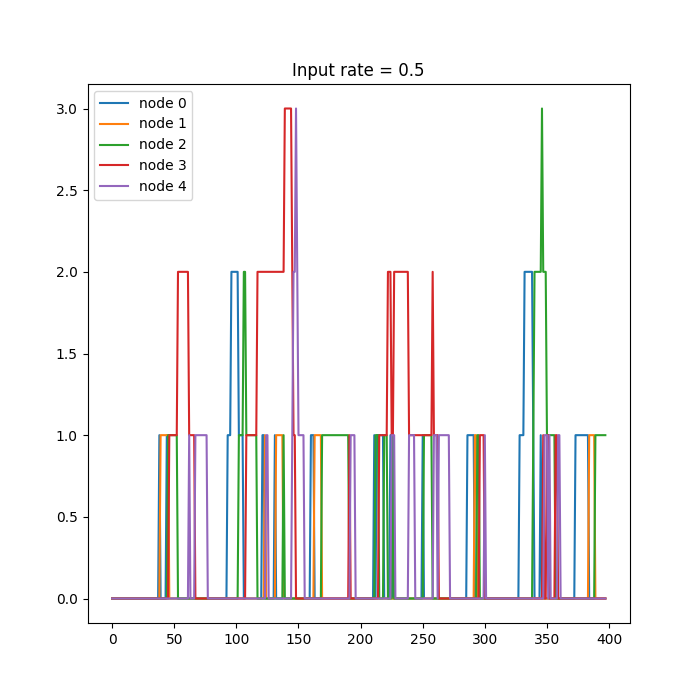
\includegraphics[width=\linewidth]{fig/fix_half}   
    \caption{number of particles at nodes in simulation}
    \label{fig:figure7}
\end{figure}

\begin{figure}[!htbp]
    \centering
    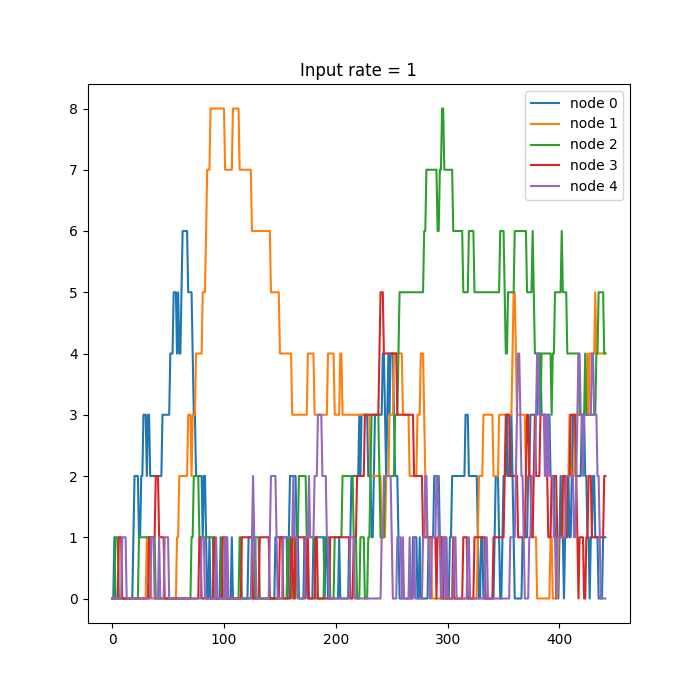
\includegraphics[width=\linewidth]{fig/fix_1}   
    \caption{number of particles at nodes in simulation}
    \label{fig:figure8}
\end{figure}

\begin{figure}[!htbp]
    \centering
    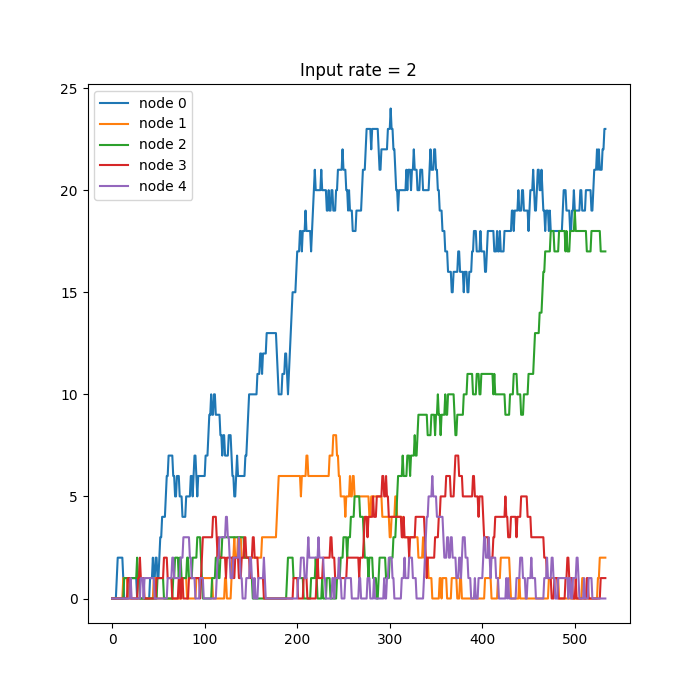
\includegraphics[width=\linewidth]{fig/fix_2}   
    \caption{number of particles at nodes in simulation}
    \label{fig:figure9}
\end{figure}









\end{document}